% Copyright 2004 by Till Tantau <tantau@users.sourceforge.net>.
%
% In principle, this file can be redistributed and/or modified under
% the terms of the GNU Public License, version 2.
%
% However, this file is supposed to be a template to be modified
% for your own needs. For this reason, if you use this file as a
% template and not specifically distribute it as part of a another
% package/program, I grant the extra permission to freely copy and
% modify this file as you see fit and even to delete this copyright
% notice. 

\documentclass{beamer}

% There are many different themes available for Beamer. A comprehensive
% list with examples is given here:
% http://deic.uab.es/~iblanes/beamer_gallery/index_by_theme.html
% You can uncomment the themes below if you would like to use a different
% one:
%\usetheme{AnnArbor}
%\usetheme{Antibes}
%\usetheme{Bergen}
%\usetheme{Berkeley}
%\usetheme{Berlin}
%\usetheme{Boadilla}
%\usetheme{boxes}
%\usetheme{CambridgeUS}
%\usetheme{Copenhagen}
%\usetheme{Darmstadt}
%\usetheme{default}
%\usetheme{Frankfurt}
%\usetheme{Goettingen}
%\usetheme{Hannover}
%\usetheme{Ilmenau}
%\usetheme{JuanLesPins}
%\usetheme{Luebeck}
\usetheme{Madrid}
%\usetheme{Malmoe}
%\usetheme{Marburg}
%\usetheme{Montpellier}
%\usetheme{PaloAlto}
%\usetheme{Pittsburgh}
%\usetheme{Rochester}
%\usetheme{Singapore}
%\usetheme{Szeged}
%\usetheme{Warsaw}
\usepackage{xcolor}
\setbeamercovered{transparent}
\usepackage{amsmath,amsfonts,amssymb}
\usepackage{eucal}
\usepackage{graphics}
\usepackage{tikz}

\defbeamertemplate*{footline}{mytheme}
{
    \leavevmode%
          \hbox{%
              \begin{beamercolorbox}[wd=.3\paperwidth,ht=2.25ex,dp=1ex,center]{section in head/foot}%
                  \usebeamerfont{author in head/foot}~{Mohammed~Khatiri}
              \end{beamercolorbox}%
              \begin{beamercolorbox}[wd=.4\paperwidth,ht=2.25ex,dp=1ex,center]{section in head/foot}%
                  \usebeamerfont{author in head/foot}~\insertshorttitle{}
              \end{beamercolorbox}%
              \begin{beamercolorbox}[wd=.3\paperwidth,ht=2.25ex,dp=1ex,right]{section in head/foot}%
                  \usebeamerfont{date in head/foot}
                  \insertframenumber{} / \inserttotalframenumber\hspace*{2ex} 
              \end{beamercolorbox}}%
                  \vskip0pt%
              }
\usebeamertemplate{mytheme}



\title{Analysis of Work Stealing with latency}

% A subtitle is optional and this may be deleted
\subtitle{Work Stealing with latency}

\author{Nicolas~Gast\inst{1} \and \textcolor{red}{Mohammed~Khatiri}\inst{1}\inst{2} \and Denis~Trystram\inst{1} \and Fr\'ed\'eric~Wagner\inst{1}}
% - Give the names in the same order as the appear in the paper.
% - Use the \inst{?} command only if the authors have different
%   affiliation.

\institute[Univ. Grenoble Alpes, CNRS, Inria, LIG] % (optional, but mostly needed)
{
    \inst{1}%
  Univ. Grenoble Alpes, France
  \and
  \inst{2}%
  University Mohammed First, Morocco}
% - Use the \inst command only if there are several affiliations.
% - Keep it simple, no one is interested in your street address.

\date{16 juin 2018 \\ \textbf{ECCO XXXI - CO 2018}}
% - Either use conference name or its abbreviation.
% - Not really informative to the audience, more for people (including
%   yourself) who are reading the slides online

%\subject{Theoretical Computer Science}
% This is only inserted into the PDF information catalog. Can be left
% out. 

% If you have a file called "university-logo-filename.xxx", where xxx
% is a graphic format that can be processed by latex or pdflatex,
% resp., then you can add a logo as follows:

% \pgfdeclareimage[height=0.5cm]{university-logo}{university-logo-filename}
% \logo{\pgfuseimage{university-logo}}

% Delete this, if you do not want the table of contents to pop up at
% the beginning of each subsection:
\AtBeginSection[]
{
    \begin{frame}<beamer>{Outline}
        \tableofcontents[currentsection]
    \end{frame}
}

% Let's get started
\begin{document}

\begin{frame}
    \titlepage
\end{frame}

\begin{frame}{Outline}
    \tableofcontents
    % You might wish to add the option [pausesections]
\end{frame}

% Section and subsections will appear in the presentation overview
% and table of contents.
\section{Context \& Related Work}

\begin{frame}{Preliminary}
    \begin{figure}
    \begin{center}
        \only<1>{ \includegraphics[width=0.7\textwidth]{Scheduling.png}}
       % \only<2->{ \includegraphics[width=0.3\textwidth]{Scheduling.png}}
    \end{center}
    \end{figure}

       \begin{center}
            \only<2->{   \textbf{Decentralized List}\\}
            \only<3->{   \textbf{\alert{Work Stealing Algorithm}}}
        \end{center}
    \begin{figure}
    \begin{center}
        \only<2> {\includegraphics[width=0.3\textwidth]{SchedulingD1.png}}
        \only<3-> {\includegraphics[width=0.3\textwidth]{SchedulingD2.png}}
        \only<3> {\includegraphics[width=0.3\textwidth]{SchedulingDS1.png}}
    \end{center}
    \end{figure}


\end{frame}


\begin{frame}{Objectives and Content}
    \begin{itemize}%[<+->]
        \item {
               Study the Work Stealing algorithm in distributed-memory platforms where communications matter. 
            }
        \item {

               Create a new realistic model for distributed-memory cluster of $p$ identical processors including communication latency. 
            }
        \item {
                Provide an upper bound of the expected Makespan.
            }
        \item {
               Provide simulation results to assess this bound. 
            }
    \end{itemize}
\end{frame}


\begin{frame}{Context}
    \begin{block}{Scheduling Problem}
        The scheduling problem is to answer the two following questions
        for each of the n independent tasks which represents an application.
        \begin{itemize}
            \item \alert{Where?} – determine the computing resources for executing each task.
            \item \alert{When?} – determined when each task will start. 

        \end{itemize}
    \end{block}
\bigskip

    \begin{itemize}
        \item \textbf{WHERE is crucial} since the load between resources must be balanced. 
        \item There are several possibilities: centralized decision, static or dynamic algorithm to determine such an assignment.

    \end{itemize}
\end{frame}



%\subsection{The classical problem}

% You can reveal the parts of a slide one at a time
% with the \pause command:
\begin{frame}{Setting of the problem}
    \begin{itemize}
        \item { Workload $\mathcal{W}$ composed of $n$ unit independent tasks.}
        \item { \emph{p} identical processors in a distributed-memory cluster.  }                                     
        \item { Each processor has its private memory}
        \item { The processors are linked by an interconnection network}                                     
    \end{itemize}
        
        \begin{block}{Makespan}
            The optimized objective is the completion time of the $n$ tasks which called the \alert{makespan} and denoted by \alert{$C_{max}$}.
        \end{block}
        
     \begin{itemize}
         \item \alert{ Communication cost between processors is most often ignored. }                                     
     \end{itemize}

\end{frame}

\begin{frame}{Classical Work Stealing algorithm}

 \begin{itemize}
     \item \textbf{Decentralized list scheduling algorithm.}
        \item { Each processor has its own queue of tasks}                                     
        \item { An active processor (defined as a non-empty tasks queue) executes tasks from its queue.}
        \item { An idle processor with empty queue (\alert{Stealer}) randomly chooses another processor (\alert{Victim}) to steal some work:}                                     
                    \pause
            \begin{itemize}
                \item {If the victim's queue is not empty, the stealer steals half of the tasks and resumes execution at \textbf{the next time slot}}
                \item {Otherwise, the stealer tries again to steal at \textbf{the next time slot}}
            \end{itemize}
        \item {If several stealers target the same victim, a random succeeds and the others fail.} 

    \end{itemize}
\end{frame}


\begin{frame}{Related Work (in brief)}
    \color{blue} {[Blumofe and Leiserson 1999, Arora et al. 2001  ]}
        \begin{itemize}        
            \item Bound the expected Makespan of a series-parallel precedence graph with $\mathcal{W}$ unit tasks on $p$ processors.
             \item $E(C_{\max}) \leq \frac{\mathcal{W}}{p}+\mathcal{O}(D)$  Where $D$ is the length of the \alert{critical path} of the graph.
        \end{itemize}  
    \color{blue} [Tchiboukdjian \textit{et al.} 2013] 
         \begin{itemize}        
             \item $\mathcal{W}$ unit independent tasks on $p$ processors (communication cost is ignored).  
             \item $E(C_{\max}) \leq \frac{\mathcal{W}}{p}+c.(\log_2 \mathcal{W})+\Theta(1)$ where $c \simeq3.24$ 
        \end{itemize}  

        \alert{Need a precise analysis of work stealing when communication is not ignored}
\end{frame}

\section{Model with communications latency}
\begin{frame}{Problem}
    \begin{alertblock}{Problem}
        \begin{itemize}
            \item When the communication cost is not ignored, the steal work takes more than one unit of time. \\
            \item The stealer takes more time to receive the answer from the victim. 
            \item The stealer must wait several time steps before receiving the answer. 
        \end{itemize}
    \end{alertblock}
    \textbf{Question :}
    \\
        What happens when the communication cost is explicit?
\end{frame} 


\begin{frame}{Model with communications cost (latency)}
  %\begin{itemize}
   %     \item {Workload $\mathcal{W}$ of $n$ unit independent tasks.}
   %    \item {Distributed-memory cluster with $p$ identical processor.}
   %     \item {Processors are linked by an interconnection network}
   %     \item {All communication between processors takes a time $\lambda$ that we called the \alert{latency}}
   % \end{itemize}
    \begin{alertblock}{Objective}
        Analyze \alert{Work Stealing} algorithm to execute a $\mathcal{W}$ workload of $n$ unit tasks on a distributed-memory cluster with $p$ identical processors and communications between them take \alert{$\lambda$} unit of times (latency).
    \end{alertblock}
\end{frame}

\begin{frame}{Work stealing algorithm with communications (latency)}
    \begin{itemize}
        \item \textbf{Principe of Work stealing (Recall)} 
            \begin{itemize}
                \item Each processor has its own queue of tasks
                \item An active processor with \textbf{not-empty} queue executes tasks from its queue
                \item When a processor becomes \textbf{idle}, it chooses randomly another processor (Victim) to steal work
            \end{itemize}
                
        \item \textbf{Latency }   
            \begin{itemize}
                \item A work request takes a time \textbf{$\lambda$ (latency)}
                \item The answer takes again $\lambda$ units of time (fail answer or work answer)
            \end{itemize}
        \item \textbf{Steal threshold:}
            \begin{itemize}
                \item If the victim has less than $\lambda$ units of work, the steal request fails.
            \end{itemize}
            
        \item \textbf{Single work transfer}
            \begin{itemize}
                \item While a victim sends some work to a stealer, it replies by a fail request to all other steal requests. 
            \end{itemize}
    \end{itemize}
\end{frame}

\begin{frame}{Analysis}
    We consider a discrete model with: 
    \begin{itemize}
        \item $p$ processors indexed by $i$ where  $i \in [1...p]$.
        \item All communications between the processors take $\lambda$ units of time.
        \item $\mathcal{W}_i(t) \in [1,2,...]$ the amount of work on processor $P_i$ at time $t$.
        \item $\mathcal{W}(t) = \sum_{i=1}^{p} \mathcal{W}_i(t)$ the total amount of Work on all the processors. 
        \item $\mathcal{S}_i(t)$ the amount of Work in transit from $P_i$ at time $t$ to another stealer. 
        \item At $t=0$ the whole work is on $P_1$ and $\mathcal{W} = \mathcal{W}_1(0)$ 
    \end{itemize}
    \bigskip
    
    \begin{block}{Theorem}
  %      Let $C_{max}$ be the Makespan. Then, deja dit...
        \begin{equation*}   
            \mathbb{E}(C_{max}) \leq \frac{\mathcal{W}}{p} +  c\lambda\log_2(\frac{\mathcal{W}}{2\lambda}) + 3\lambda
        \end{equation*}             where $c \leq 16.12$ 
    \end{block}
\end{frame}

\section{Analysis}
\begin{frame}{Principle of the analysis (1)}
    \begin{columns} 
        \column{0.45\textwidth} 
        \begin{center}
            \includegraphics[width=1\textwidth]{ws.pdf}
        \end{center}
        \column{0.55\textwidth} 
        \begin{center} 
            $pC_{\max} \le \mathcal{W} + 2\lambda\#\textit{StealRequests}$
%            Where $\mathcal{W}, p, \lambda$ are the total amount of work, the total number of processors and the communication latency respectively. 
        \end{center} 
        \begin{equation}
            C_{max}  \leq \frac{\mathcal{W}}{p} + 2\lambda\frac{\#StealRequests}{p}
        \end{equation} 
    \end{columns} 
    \begin{center}
    To bound \alert{$C_{max}$}, we need to bound \alert{$\#StealRequests$}
    \end{center}
\end{frame}


\begin{frame}{Principle of the analysis (2)}
    The analysis is based on a \textbf{potential function} that represents \textit{how well the jobs are balanced in the system}.
    \begin{block}{Potential function}
    Our potential function \textbf{at time-step \alert{$k\lambda$}} is denoted by $\phi(k)$ and : %it is defined as:
    \begin{equation*}
        \phi(k) = \sum_{i=1}^{p} \phi_i(k),  
        \text{ where $\phi_i(k) =
         \mathcal{W}_{i}(k\lambda)^{2} + 2\mathcal{S}_{i}(k\lambda)^{2}$ \quad for $i\in\{1\dots,p\}$}. 
    \end{equation*}
    \end{block}
    \begin{columns} 
        \column{0.55\textwidth} 
    \textbf{Properties}
    \begin{itemize}
        \item Always decreases. 
        \item Its maximal at time 0, $\phi(0)= \mathcal{W}^2$
        \item Becomes $0$ at the end of schedule. 
        \item Decreases according to each processor event (executing work, sending or answering steal request) 
    \end{itemize}
        \column{0.45\textwidth} 
    \textbf{Analysis method}\\

    \alert{ We analyse how much each case contributes to the decrease of the potential between \alert{$\lambda k$} and \alert{$\lambda(k+1)$}}
    \end{columns}
\end{frame}
\begin{frame}{Principle of the analysis (3)}

\begin{alertblock}{Lemme 1}
    We denote by $\mathcal{F}_{k}$ all events up to the interval $((k-1)\lambda$, $\lambda k$]

        For all steps $k$, the expected ratio between $\phi(k+1)$ and $\phi(k)$ knowing $\mathcal{F}_{k}$ is bounded by: 
        \begin{equation*}
            \mathbb{E}[\phi(k+1) \:|\: \mathcal{F}_{k}] \leq \left(1-\frac{q(r_k)}{4}\right)\phi(k) 
            \label{expdiff}
        \end{equation*}


        Where $q(r_k)$ is the probability for a processor to receive one
        or more steal requests in the interval $((k-1)\lambda,k\lambda]$ knowing that there are $r_k$ incoming steal requests.
        \begin{equation*}
            q(r_k) = 1 - \left(\frac{p-2}{p-1}\right)^{r_k}
            \label{expdiff}
        \end{equation*}
       % The worst case of $q(r_k)$ is maximal when all the processors send a steal request ($r_k=p-1$)
        
        \end{alertblock}
\end{frame}


    \begin{frame}{Principle of the analysis (4)}

        \begin{itemize}
            \item Using :
        \begin{itemize}
            \item The potential function at time 0 \alert{($\mathcal{W}^2$)} and at the end of schedule \alert{(0)}
            \item The result of lemme 1.
        \end{itemize}
    \item We bound the expected number of steal request between $0$ and the end of schedule.
                
    \item Then, we derive the bound of the expected makespan $C_{max}$ using the equation:
        \begin{equation*}
            C_{max}  \leq \frac{\mathcal{W}}{p} + 2\lambda\frac{\#StealRequests}{p}
        \end{equation*} 
        \end{itemize}
\end{frame}

\section{Experimental Results}
\begin{frame}{Experimental Results}

        \begin{equation*}   
            \mathbb{E}(C_{max}) \leq \alert{\frac{\mathcal{W}}{p}} +  c\lambda\log_2(\frac{\mathcal{W}}{2\lambda}) + 3\lambda
        \end{equation*}             
       $ \alert{\frac{\mathcal{W}}{p}} $ \alert{does not depend on the configuration and the algorithm }
\pause
    \begin{equation*}
        \text{ Overhead ratio = } \frac{c\lambda\log_2(\mathcal{W}/2\lambda) + 3\lambda}{Simulation Time - \mathcal{W}/p} 
    \end{equation*}
\pause

    \textbf{Simulator : }
    \begin{itemize}
        \item A python discrete event simulator.
        \item The simulator follows the model described to schedule an amount $\mathcal{W}$ of work on a distributed platform with $p$ identical processors 
        \item The communication cost is equal to the latency $\lambda$
    \end{itemize}
    \textbf{Configuration}
    \begin{itemize}
        \item  $ 10^5 \leq \alert{\mathcal{W}} \leq 10^8$
            , $ 32 \leq \alert{p} \leq 256$ and  
            $ 2 \leq \alert{\lambda} \leq 500$ 
        \item Each experiment has been reproduced \alert{$1000$} times
    \end{itemize}
\end{frame}

%\begin{frame}{Experimental Results}
 %   \begin{figure}
%        \only<1> {       \includegraphics[width=0.7\textwidth]{OV-eps-converted-to.png}}
  %      \includegraphics[width=0.7\textwidth]{OV-eps-converted-to-1.png}
   %     \caption{Overhead ratio as a function of $(\mathcal{W},p)$
    %            ($\lambda = 262$)} \label{fig:accuracy}
   % \end{figure}
%\end{frame}

\begin{frame}{Experimental Results}

        \begin{figure}
            %        \only<1> {       \includegraphics[width=0.7\textwidth]{OV-eps-converted-to.png}}
            \includegraphics[width=0.7\textwidth]{OV-eps-converted-to-1.png}
            \caption{Overhead ratio as a function of $(\mathcal{W},p)$
                ($\lambda = 262$)} \label{fig:accuracy}
        \end{figure}
        \begin{center}
        \textbf{Similar observations have been observed with all values of latency used}
        \end{center}

\end{frame}


\begin{frame}{Experimental Results}

    \begin{columns} 
        \column{0.5\textwidth} 
        \begin{figure}
            %        \only<1> {       \includegraphics[width=0.7\textwidth]{OV-eps-converted-to.png}}
            \includegraphics[width=1\textwidth]{OV-eps-converted-to-1.png}
        \end{figure}
            \column{0.5\textwidth} 
            \textbf{Observations}
            \begin{itemize}
                \item Our bound is about \alert{$4$} to \alert{$5.5$} times greater to the one computed by simulation  
                    \pause
                \item [\scriptsize\raise1.25pt\hbox{\donotcoloroutermaths$\blacktriangleright$}] 
                    \alert{Because we take the worst case in different cases of the analysis}  
                    \pause
                \item The ratio decrease with the number of processors \textbf{but seems fairly independent to $\mathcal{W}$ }
            \end{itemize}
    \end{columns}
            \begin{itemize}
                    \pause
                  \item  [\scriptsize\raise1.25pt\hbox{\donotcoloroutermaths$\blacktriangleright$}]
                      \alert{Because in the theoretical bound of the second term, we major the number of processors,
                      which makes the born independent to the number of processors, 
                      but it still reacted on the simulation results. }
            \end{itemize}

\end{frame}

 \section{Conclusion}
    \begin{frame}{Conclusion and Perspective}
        \textbf{Conclusion}
            \begin{itemize}
                \item Created a new realistic scheduling model for distributed-memory cluster of $p$ identical processors including latency $\lambda$
                \item Analyzed this model and provide an upper bound of the Makespan  
                \item Provided simulation results to assess this bound. 
            \end{itemize}

            \textbf{Perspective}

            \hspace{0.3cm}    This work forms the basis of incoming studies on more complex

            \hspace{0.3cm} hierarchical topologies :

            \begin{itemize}
                \item Communication cost inside clusters is small
                \item Communication cost outside clusters is important
            \end{itemize}

    \end{frame}


\begin{frame}
    \begin{center}
                Our paper is available on Arxiv : https://arxiv.org/abs/1805.00857 \\ 
                E-mail : \alert{khatiri.med@gmail.com}\\
    \end{center}

    \begin{center}
        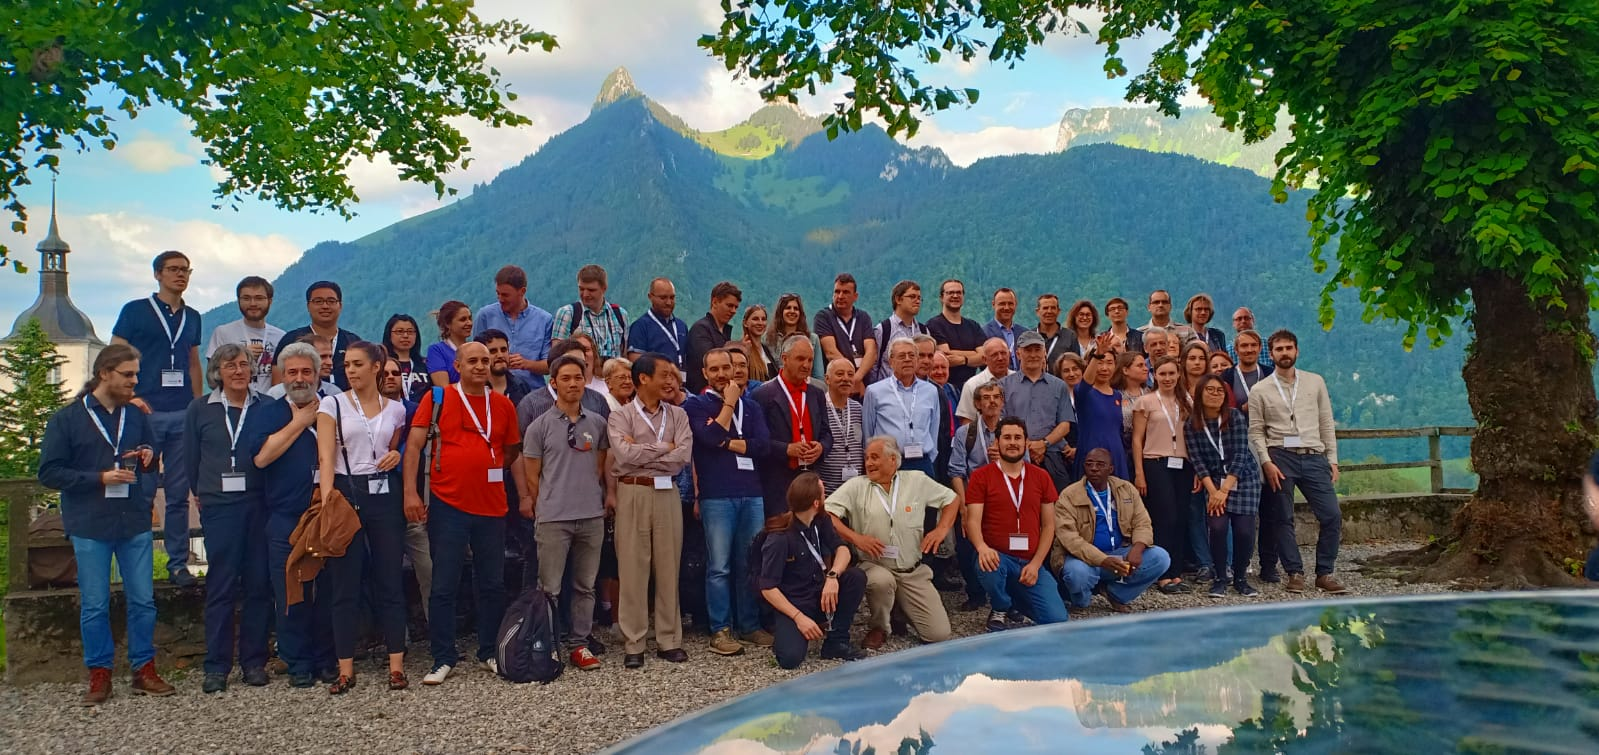
\includegraphics[width=0.7\textwidth]{ECCO.jpeg} 

                Tank you,
    \end{center}
\end{frame}



    % Placing a * after \section means it will not show in the
    % outline or table of contents.


\end{document}



